\documentclass{article}
\usepackage{pgf-pie}
\usepackage{pgfplots}

\begin{document}

\begin{figure}
  \centering
  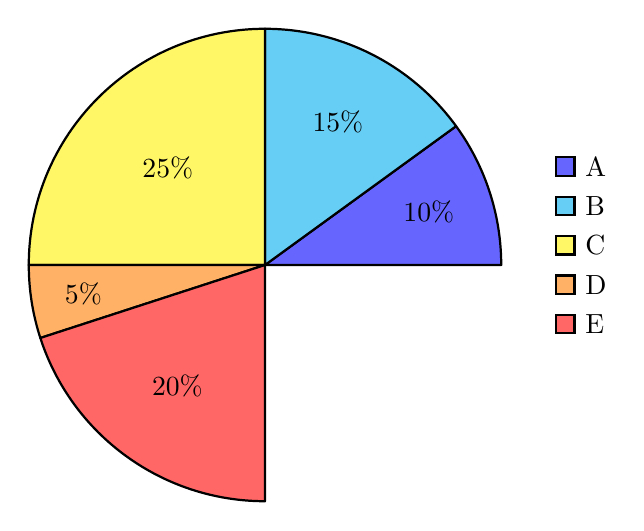
\begin{tikzpicture}
    \pie[text=legend]{10/A, 15/B, 25/C, 5/D, 20/E}
  \end{tikzpicture}
  
  \vspace{1cm}
  
  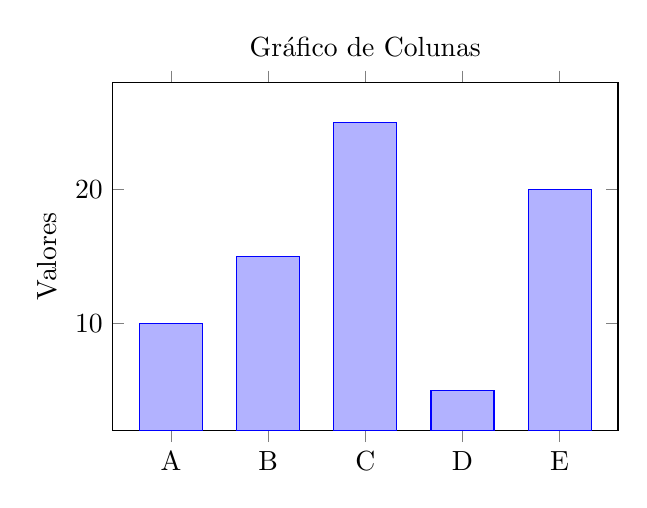
\begin{tikzpicture}
    \begin{axis}[
        title={Gráfico de Colunas},
        symbolic x coords={A,B,C,D,E},
        ylabel={Valores},
        enlargelimits=0.15,
        legend style={at={(0.5,-0.15)},
        anchor=north,legend columns=-1},
        ybar,
        width=8cm,
        height=6cm,
        bar width=0.8cm,
      ]
      \addplot coordinates {(A,10) (B,15) (C,25) (D,5) (E,20)};
    \end{axis}
  \end{tikzpicture}
  
  \caption{Exemplo de gráficos de pizza e colunas.}
\end{figure}

\end{document}

